
\documentclass[12pt, a4paper]{article}

\usepackage[utf8]{inputenc}
\usepackage[T1]{fontenc}
\usepackage[russian]{babel}
\usepackage[oglav,spisok,boldsect,eqwhole,figwhole,hyperref,hyperprint,remarks,greekit]{./style/fn2kursstyle}
\graphicspath{{./style/}{./figures/}}

\usepackage{multirow}
\usepackage{supertabular}
\usepackage{multicol}
\usepackage{amsmath}
\usepackage{afterpage}
% Параметры титульного листа
\title{Упругие характеристики поликристаллических металлов \\ Вариант 15 \\ $Si+Mg$}
\author{В.\,Г.~Пиневич}
\supervisor{Е.\,А.~Максимова}
\group{ФН2-71Б}
\date{2023}

% Переопределение команды \vec, чтобы векторы печатались полужирным курсивом
\renewcommand{\vec}[1]{\text{\mathversion{bold}${#1}$}}%{\bi{#1}}
\newcommand\thh[1]{\text{\mathversion{bold}${#1}$}}
%Переопределение команды нумерации перечней: точки заменяются на скобки
\renewcommand{\labelenumi}{\theenumi)}
\begin{document}

\maketitle

\tableofcontents



\newpage

\section-{Список условных обозначений}

\noindent\begin{tabular}{cp{0.7\textwidth}}
	
	$C$ & --- матрица коэффициентов упругости \\
	$C_{ij}$ & --- элементы матрицы $C$ $(i, j = \overline{1,6})$ \\
	$S$ & --- матрица коэффициентов податливости \\
	$S_{ij}$ & --- элементы матрицы $S$ $(i, j = \overline{1,6})$ \\
	%$\vec{n} = \{n_1,n_2,n_3\}$ & --- единичный %вектор нормали, заданный в кристаллографических %осях. Компоненты $n_i$ --- проекции на $Ox^'_i$ \\
	$S_n$ & --- линейная податливость в направлении $\vec{n}$ \\
	$e^{(\vec n)}$ &--- относительное удлинение в направлении $\vec n$\\
	$\sigma_{kl}$ & ---  компоненты тензора напряжений $\hat{\sigma}$ $(k, l = \overline{1,3})$\\
	$S_{ijkl}$ & --- компоненты тензора податливости $\hat{S}$ $(i, j,k,l = \overline{1,3})$ \\
	$\varepsilon_{kl}$ & --- компоненты тензора малой деформации $\hat{\varepsilon}$ $(k, l = \overline{1,3})$\\
	$p$ & --- давление\\
	$\delta_{ij}$ & --- символ Кронекера \\
	$V_0$ & --- контрольный объем\\
	$I_{ijkl}$ & --- единичный тензор 4-го ранга $(i, j,k,l = \overline{1,3})$\\
	$\nu$ & --- коэффициент Пуассона\\
	$C_{ijkl}$ & --- компоненты тензора коэффициентов упругости $\hat{C}$ $(i, j,k,l = \overline{1,3})$ \\
	$C^o_{ijkl}$ & --- эффективные упругие характеристики поликристалла $(i, j,k,l = \overline{1,3})$ \\
	$S^o_{ijkl}$ & --- эффективные характеристики податливости поликристалла $(i, j,k,l = \overline{1,3})$ \\
	$\omega_{ijkl}$ & --- тензор Эшелби $(i, j,k,l = \overline{1,3})$\\
	$E$ & --- модуль Юнга, ГПа\\
	$\mu$ & --- модуль сдвига, ГПа\\
	$\kappa$ & --- модуль объемной упругости, ГПа
\end{tabular}

\newpage

\section{Постановка задачи}

Для заданной пары чистых металлов по значениям коэффициентов упругости
(или податливости) кристаллов вычислить элементы матрицы коэффициентов податливости (или упругости), сравнив точность обращения матриц с вычислением по
формулам, и построить графики зависимостей линейной податливости от направления единичного вектора для гексагональной кристаллической решетки в плоскости,
содержащей оптическую ось кристалла, а для кубической кристаллической решетки в плоскости грани и в плоскостях, 
имеющие общую точку диагонали двух граней,
 диагонали грани и куба, диагональ куба и ребро. Для
кристаллической решетки каждого из металлов определить направления, по которым линейная податливость имеет экстремальные значения. Найти отношение полуосей эллипсоида вращения, образующегося после действия всестороннего давления
на шар из металла с ГПУ кристаллической решеткой.

Для каждого из металлов в предположении хаотической ориентации зерен в поликристалле найти верхнюю и нижнюю оценки модулей сдвига, продольной и объемной
упругости, оценки коэффициента Пуассона и сравнить полученные значения с вычисленными для случая статистически усредненной шаровой формы кристаллических
зерен. Провести аналогичные расчеты и построить графики для пористого двухфазного сплава-смеси заданной пары металлов при трех фиксированных значениях объемной пористости, равных 0; 0.1 и 0.2, в зависимости от отношения $\dfrac{V_1}{(V_1+V_2)}\in [0;1]$, где $V_1$ и $V_2$ --- объемные доли металлов в сплаве.

\begin{table}[htb!]
	\centering	
	\caption{Коэффициенты упругости и податливости}
	\vspace*{3mm}
	\begin{tabular}{|c|c|c|c|}
		\hline
		$Si$ & $C_{11}$ & $C_{12}$ & $C_{44}$ \\
		\hline
		ГПа & 167 & 61 & 76 \\
		\hline
	\end{tabular}
	\qquad
	\begin{tabular}{|c|c|c|c|c|c|}
		\hline
		$Mg$ & $S_{11}$ & $S_{12}$ & $S_{13}$ & $S_{33}$ & $S_{44}$ \\
		\hline
		TПа$^{-1}$ & 23.9 & -9.48 & -5.36 & 20.9 & 70.4 \\
		\hline
	\end{tabular}
	\label{tab1}
\end{table}

\newpage

\section-{Вычисление элементов матриц коэффициентов
	упругости и коэффициентов податливости}

Соотношение для связи коэффициентов упругости и коэффициентов податливости
\[
C_{ijmn} S_{mnkl} = I_{ijkl}.
\]
В матричной форме записи тензоров 4 ранга $\hat{C}, \hat{S}$ это выражение будет иметь вид 
\begin{equation}
	\label{matr_C-S_form}
	\hat{C} \hat{S} = I
\end{equation}

\subsection{Матрицы податливости и упругости для кубической кристаллической решетки}
В кристаллах с кубической решеткой все оси $Ox_k$ равноправны и матрица S коэффициентов податливости содержит лишь три отличных от нуля независимых элемента
\[
S=
\begin{pmatrix}
	S_{11} & S_{12} & S_{12} & 0 & 0 & 0\\
	S_{12} & S_{11} & S_{12} & 0 & 0 & 0\\
	S_{12} & S_{12} & S_{11} & 0 & 0 & 0\\
	0 & 0 & 0 & S_{44} & 0 & 0\\
	0 & 0 & 0 & 0 & S_{44} & 0\\
	0 & 0 & 0 & 0 & 0 & S_{44} 
\end{pmatrix}.  
\]
Матрица коэффициентов упругости $C$ имеет аналогичный вид.
Найдем коэффициенты податливости используя формулы из источника~\cite{first-zarubin} и проведя расчеты в с помощью Wolfram Mathematica.

\begin{gather*}
	S_{11} = \frac{C_{11} + C_{12}}{C_K}, S_{12} = - \frac{C_{12}}{C_K}, S_{44} = \frac{1}{C_{44}},
\end{gather*}
где $C_K = C_{11}^2 + C_{11} C_{12} - 2 C^2_{12}$.

Теперь определим коэффициенты податливости при помощи матрицы $C$ из~(\ref{matr_C-S_form}). Получаем 
\begin{gather*}
	S_{11} = 7.44 \text{ ТПа}^{-1}, S_{12} = 1.99 \text{ ТПа}^{-1}, S_{33} = 1.32 \text{ ТПа}^{-1}.
\end{gather*}
Норма ошибки:
\[
\| S - C^{-1} \| = 2 \cdot 10^{-27}.
\]

\subsection{Матрицы податливости и упругости для гексагональной кристаллической решеткой}
 
Кристаллы с ГПУ-решеткой обладают высокой степенью симметрии относительно кристаллографической оси $Ox_3$. Поэтому их упругие свойства в плоскости, перпендикулярной этой оси, изотропны, а матрица S коэффициентов податливости включает пять независимых ненулевых элементов:
\[
S=
\begin{pmatrix}
	S_{11} & S_{12} & S_{13} & 0 & 0 & 0\\
	S_{12} & S_{11} & S_{13} & 0 & 0 & 0\\
	S_{13} & S_{13} & S_{33} & 0 & 0 & 0\\
	0 & 0 & 0 & S_{44} & 0 & 0\\
	0 & 0 & 0 & 0 & S_{44} & 0\\
	0 & 0 & 0 & 0 & 0 & S_{66} 
\end{pmatrix}.  
\]
Коэффициент $S_{66} = \frac{S_{11} - S_{12}}{2}$.

Действуя аналогично с прошлым пунктом найдем коэффициенты упругости используя формулы из источника~\cite{first-zarubin}.

\begin{gather*}
	C_{11} = \frac{S_{33}}{2 S_{h}} + \frac{1}{2 \left( S_{11} - S_{12} \right)}, 
	C_{12} = \frac{S_{33}}{2 S_{h}} + \frac{1}{2 \left( S_{11} - S_{12} \right)},
	C_{13} = -\frac{S_{33}}{2 S_{h}},\\
	C_{33} = \frac{S_{11} + S_{12}}{2 S_{Г}},
	C_{44} = \frac{1}{S_{44}},
	C_{66} = \frac{1}{2 \left( S_{11} - S_{12} \right)
	}
\end{gather*}
где $S_h = \left(S_{11} + S_{12}\right) S_{33} - 2 S_{12}^2$.

Теперь определим коэффициенты податливости при помощи матрицы $S$ из~(\ref{matr_C-S_form}). Получаем 
\begin{gather*}
	C_{11} = 57.82 \text{ ГПа},
	C_{12} = 27.86 \text{ ГПа},
	C_{13} = 21.97 \text{ ГПа},\\
	C_{33} = 59.12 \text{ ГПа},
	C_{44} = 14.20 \text{ ГПа},
	C_{66} = 14.98 \text{ ГПа}.
\end{gather*} 
Норма ошибки:
\[
\| C - S^{-1} \| = 1.5 \cdot 10^{-5}.
\]

\section{Линейная податливость}
Пусть на кристалл действует внешнее растягивающее напряжение $\sigma_{kl} = \sigma n_k n_l$ в направлении $\vec{n} = \{n_1, n_2, n_3  \}$. Тогда линейная податливость в направлении действия
напряжения имеет вид
\[
S_N = \frac{e^{(\vec{n})}}{\sigma} = S_{ijkl} N_i n_j n_k n_l,
\]
где $e^{(\vec{n})}$ --- относительное удлинение материла в направлении $\vec{n}$.

\subsection{Линейная податливость для металлов с кубической кристаллической решеткой}

Линейная податливость для металлов с кубической кристаллической решеткой
равна 
\begin{gather} 
	\label{2-1_kub-resh-lin}
	S_N = S_{11} - \left( 2 \left(S_{11} - S_{12}\right) - S_{44} \right) (n_1^2 n_2^2 + n_1^2 n_3^2 + n_2^2 n_3^2).
\end{gather}

Получим зависимость линейной податливости $S_n$ от направления единичного вектора, лежащего в плоскости грани куба. Рассмотрим грань куба, лежащую в плоскости $O x_1 x_2$, на которой $n_3 = 0$ (для других граней куба аналогично). Учитывая равенство
\[
n_1^2 + n_2^2 + n_3^2 = 1
\]
получаем $n_2^2 = 1 - n_1^2$. Тогда соотношение~(\ref{2-1_kub-resh-lin}) будет выглядеть следующим образом
\[
S_n = S_{11} - \left( 2 \left(S_{11} - S_{12}\right) - S_{44} \right) n_1^2 \left(1 - n_1^2\right).
\]
График функции $S_n$ в плоскости грани куба в зависимости от $n_2$ изображен
на рис.~\ref{lin-pod-kube}. В плоскости грани куба линейная податливость минимальна в направлении диагонали грани, и
максимальна в направлениях параллельных граням.
\begin{figure}[!htbp]
	\centering
	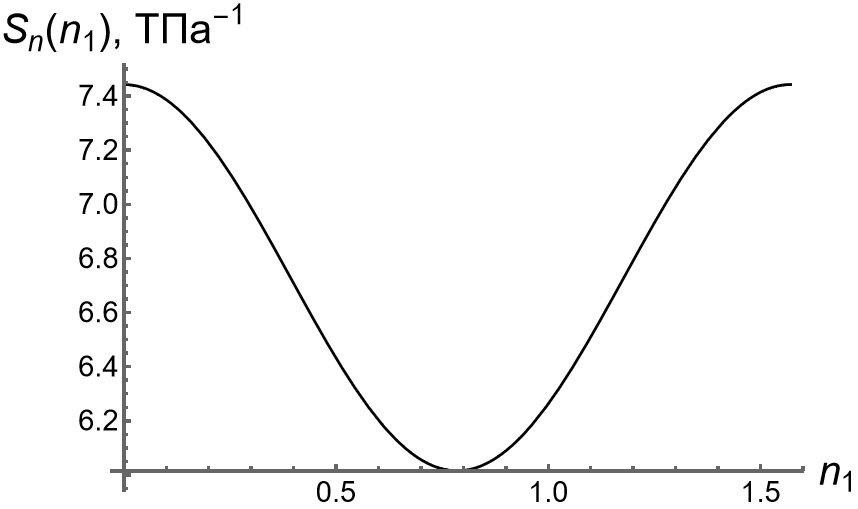
\includegraphics[width=0.8\textwidth]{pic-1}%
	\caption{Линейная податливость в плоскости грани куба}
	\vspace*{-2mm}
	\label{lin-pod-kube}
\end{figure}

Теперь найдем зависимость линейной податливости $S_n$ от направления единичного вектора, лежащего в плоскостях, содержащих диагонали грани и куба. Пусть
диагональ грани лежит в плоскости $Ox_1x_2 \left(x_1 = x_2 \right)$.
Тогда получаем равенства\\
$n_{3}^{2} = 1 - n_{1}^{2} - n^2_2$,
$n_1 = n_2$. Тогда соотношение~(\ref{2-1_kub-resh-lin}) имеет вид
\[
S_n = S_{11} - \left( 2 \left(S_{11} - S_{12}\right) - S_{44} \right) n_1^2 \left(2 - 3 n_1^2\right)
\]

График функции $S_n$ в плоскостях, содержащих диагонали грани и куба в зависимости от $n_1$ представлен на рис. 2. Линейная податливость минимальна в направлении диагонали куба, и
максимальна в направлении, параллельном грани куба.
\begin{figure}[!htbp]
	\centering
	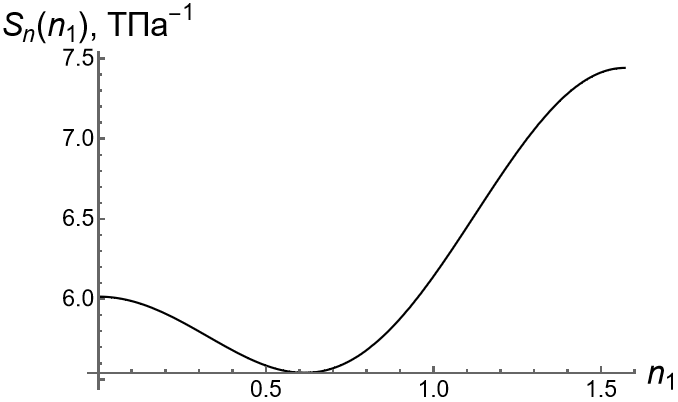
\includegraphics[width=0.8\textwidth]{pic-2}%
	\caption{Линейная податливость в плоскостях, содержащих диагонали грани и куба}
	\vspace*{-2mm}
	\label{lin-grani-kuba}
\end{figure}

Вычислим направления максимальной податливости и минимальной линейной податливости. Воспользуемся функциями Maximize и Minimize Wolfram Matematica для этого. В результате расчетов получим, что максимальное значение функции $S_N(n_1, n_2, n_3)$ в направлении вектора $\vec{n} = \{1, 0, 0\}$, т.е. в направлении грани куба, а минимальное значение функции при координатах вектора $\vec{n}$ равных $n_1 = n_2 = n_3 = \frac{\sqrt{3}}{3}$, что соответствует направлению диагонали куба.

Теперь найдем зависимость линейной податливости $S_n$ от направления единичного вектора, лежащего в плоскостях, содержащих диагонали двух граней, имеющих общую точку.

В плоскости, содержащей диагонали грани в плоскости $O x_1 x_3$ и $O x_2 x_3$: 
\[
n_1 - n_2 + n_3 = 0; n_1^2 + n_2^2 + n_3^2 = 1 \text{, тогда}
\]
\[
S_n = S_{11} - \frac{\Delta{S}}{4}.
\]

\begin{figure}[!htbp]
	\centering
	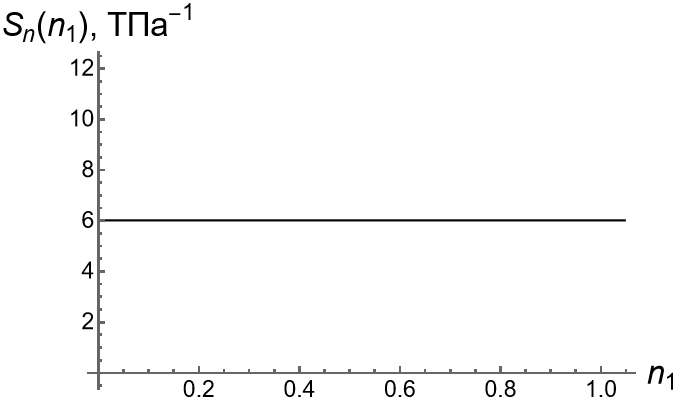
\includegraphics[width=0.8\textwidth]{pic-5}%
	\caption{Линейная податливость в плоскостях, содержащих диагонали двух граней}
	\vspace*{-2mm}
	\label{lin-grani-2-kuba}
\end{figure}
\newpage

 Получаем, что графиком функции является прямая, параллельная оси абсцисс. Полученный результат закономерен, так как $n_1^2 n_2^2 + n_2^2 n_3^2 + n_3^2 n_1^2 = \dfrac{1}{4}$.
 
 Теперь найдем зависимость линейной податливости $S_n$ от направления единичного вектора, лежащего в плоскостях, содержащих диагональ куба и ребро, имеющих общую точку.
 
В плоскости, содержащей диагонали грани в плоскости $O x_2 x_3$ и куба: 
\[
n_2 = n_3; n_1^2 + n_2^2 + n_3^2 = 1 \text{, тогда}
\]
\[
S_n = S_{11} - \frac{\Delta{S}}{4} \left(1 - n_1^2\right) \left(1 + 3 n_1^3\right).
\]
 \begin{figure}[!htbp]
 	\centering
 	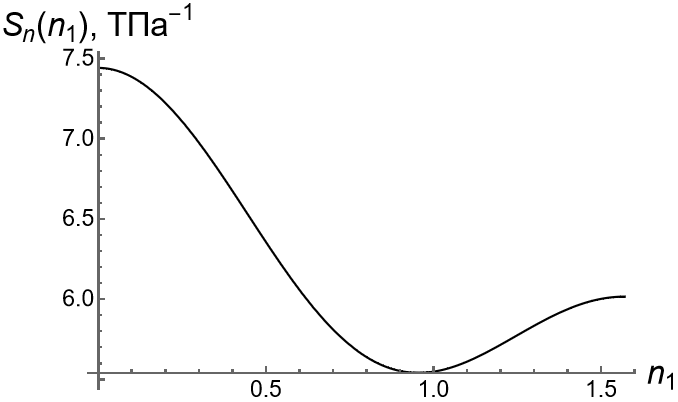
\includegraphics[width=0.5\textwidth]{pic-6}%
 	\caption{Линейная податливость в плоскостях, содержащих диагональ куба и ребро}
 	\vspace*{-2mm}
 	\label{lin-grani-2-kuba}
 \end{figure}

\newpage

\subsection{Линейная податливость для металлов с гексагональной кристаллической решеткой}
Линейная податливость кристалла с ГПУ-решеткой зависит лишь от угла между
направлением действия силы и осью $Ox_3:$
\begin{gather}
	\label{lin-geks-form}
S_n = S_{11} \left(1 - n_3^2\right)^2 + S_{33} n_3^4
 + (2 S_{13} + S_{44}) (1 - n^2_3)n^2_3
\end{gather}
График зависимости линейной податливости от направления единичного вектора
в плоскости, содержащей оптическую ось кристалла, представлен на рис.~\ref{lin-pod-v-plock-krsit-pic-4}. линейная податливость минимальна в направлении оптической оси и максимальна при
$n3 \approx 1$.
\begin{figure}[!htbp]
	\centering
	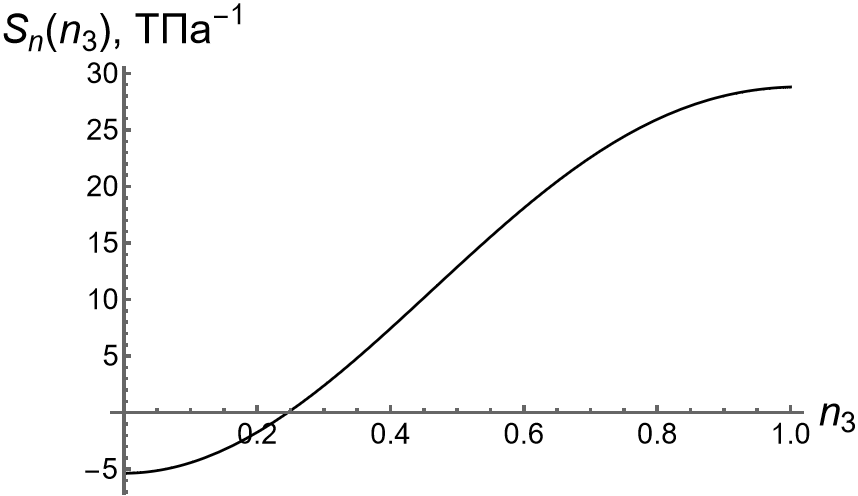
\includegraphics[width=0.8\textwidth]{pic-4}%
	\caption{Линейная податливость в плоскости, содержащей оптическую ось кристалла}
	\vspace*{-2mm}
	\label{lin-pod-v-plock-krsit-pic-4}
\end{figure}

\section{Деформирование шара из металла с ГПУ кристаллической решеткой при всестороннем давлении}

Рассмотрим задачу действия всестороннего давления на шар из $Mg$. Найдем отношение полуосей эллипсоида вращения, образующегося после данного воздействия.
Из условия всестороннего давления $p$ имеем $\sigma_{kl} = - p \beta_{kl}$.
Деформация в направлении вектора имеет вид $e^{(\vec{n})} = \varepsilon_{ij}n_in_j$.
Учитывая выражение $\varepsilon_{ij} = S_{ijkl}\sigma_{kl}$, для металла
с гексагональной решеткой имеем
\begin{gather*}
e^{(\vec{n})} = S_{klmn} \sigma_{mn} n_K n_l = - p S_{klmn} \beta_{mn} n_k n_l = - p S_{klmm} n_k n_l = - p S_{kkmm}n_p n_p;\\
e^{(\vec{n})} = -p \left(\left(S_{11} + S_{12} + S_{13} \right)n_1^2 + \left(S_{11} + S_{12} + S_{13} \right)n_2^2 + \left(S_{13} + S_{33} + S_{13} \right)n_3^2 \right);\\
e^{(\vec{n})} = -p \left( \left( S_{11} + S_{12} + S_{13}\right) + \left( S_{33} + S_{13} - S_{11} - S_{12}\right) \right)
\end{gather*}
Изменение полуоси в направлении вектора $n_3$ имеет вид
\[
a = - p \left( \left( S_{11} + S_{12} + S_{13}\right) + \left( S_{33} + S_{13} - S_{11} - S_{12}\right) \right),
\]
а в направлении, перпендикулярном $n_3$:
\[
b = -p  \left( S_{11} + S_{12} + S_{13}\right).
\]
Следовательно, отношение полуосей эллипсоида вращения равняется
\[
\frac{a}{b} \approx 1.12
\]

\section{Оценки коэффициента Пуассона}
Значения коэффициента Пуассона можем найти из соотношения 
\begin{gather}
	\label{puasson-4}
	\nu = \frac{\kappa / 2 - G / 3}{\kappa + G / 3}
\end{gather}

\subsection{Оценки по Фойгту и по Рейссу}
Для нахождения верхних оценок для модуля сдвига и модуля всестороннего сжатия по Фойгту будем считать, что в поликристаллическом материале деформация одинакова во всех зернах ($\bar{\varepsilon}_{ij} = \varepsilon_{ij}^{\circ} = const$).
Для минимизируемого функционала Лагранжа такие распределения перемещений являются допустимыми. Этот функционал в таком случае принимает вид
\[
J[\varepsilon_{ij}] = \frac{1}{2} \int \limits_{V_0} {C_{ijmn (M} \varepsilon_{mn} (M) \varepsilon_{ij} (M) d V}.
\]

Действительным распределениям перемещений в представительном объеме $V_0$ соответствует истинное распределение $\varepsilon_{ij}^{*} (M)$ компонент тензора деформации, на котором функционал $J[\varepsilon_{ij}]$ принимает минимальное значение.
Задача минимизации $J[\varepsilon_{ij}]$ приводит к решению системы неравенств
\[
\begin{cases}
	C_{kkmm} - C_{kkmm}^{\circ} \leq 0,\\
	C_{klkl} - C_{klkl}^{\circ} \leq 0
\end{cases}
\]

откуда получаем верхние оценки для модуля сдвига $G^+$ и модуля всестороннего сжатия $\kappa^+$.
На истинном распределении напряжений в представительном объеме $V_0$ функционал.

Для нахождения нижних оценок для модуля сдвига и модуля всестороннего сжатия по Рейссу будем считать, что в поликристаллическом материале напряжения одинаковы во всех зернах ($S_{ij} = S_{is}^{\circ} = const$). Для минимизируемого функционала Кастилиано такие распределения перемещений являются допустимыми. Этот функционал в таком случае принимает вид
\[
I[\sigma i j] = - \frac{1}{2} \int \limits_{V_0} {S_{ijmn} (M) \sigma_{mn} (M) \sigma_{ij} (M) dV}
\]
На истинном распределении напряжений в представительном объеме $V_0$ функционал $I[\sigma i j]$ принимает максимальное значение.
Задача максимизации $I[\sigma i j]$ приводит к решению системы неравенств
\[
\begin{cases}
	S_{kkmm} - S_{kkmm}^{\circ} \leq 0,\\
	S_{klkl} - S_{klkl}^{\circ} \leq 0
\end{cases}
\]
откуда получаем нижние оценки для модуля сдвига $G^{-}$ и модуля всестороннего сжатия $\kappa^{-}$.

Таким образом, оценки модуля сдвига и модуля всестороннего сжатия для кубической кристаллической решетки имеют вид
\[
G^{-} = \frac{5}{4 S_{11} + 3 S_{44} - 4 S_{12}},
G^{+} = \frac{C_{11} - C_{12} + C_{44}}{5},
\kappa^{-} = \frac{1}{3 (S_{11} + 2 S_{12})} = \frac{C_{11} + 2 C_{12}}{3} = \kappa^{+}
\]
Тогда оценки для коэффициента Пуассона для кубической кристаллической решетки
имеют вид
\[
v_{-} = \frac{\kappa^{+} / 2 - G^{+} / 3}{\kappa^{+} + G^{+} / 3} = 0.2184,
v_{+} = \frac{\kappa^{-} / 2 - G^{+} / 3}{\kappa^{-} + G^{-} / 3} = 0.2184
\]
Оценки модуля сдвига и модуля всестороннего сжатия для ГПУ-решетки:
\begin{gather*}
	G^{-} = \frac{15}{2(7 S_{11} + 2 S_{33} - 5 S_{12} + 3 S_{44} - 4 S_{13})},\\
	G^{+} = \frac{7 C_{11} + 12 C_{44} - 5 C_{12} + 2 C_{33} - 4 C_{13}}{30},\\
	\kappa^{-} = \frac{1}{2 S_{11} + S_{33} + 2 S_{12} + 4 S_{13}},\\
	\kappa^{+} = \frac{2 C_{11} + C_{33} + 2 C_{12} + 4 C_{13}}{9},
\end{gather*}
Тогда оценки для коэффициента Пуассона для ГПУ-решетки имеют вид
\[
v_{-} = \frac{\kappa^{+} / 2 - G^{+} / 3}{\kappa^{+} + G^{+} / 3} = 0.3084,
v_{+} = \frac{\kappa^{-} / 2 - G^{+} / 3}{\kappa^{-} + G^{-} / 3} = 0.3104,
\nu^{-} \leq \nu \leq \nu^{+}.
\]
\subsection{Задача Эшелби}
Для оценки характеристик поликристаллического материала можно использовать решение задачи Эшелби о взаимодействии с изотропной линейно-упругой сплошной средой изотропного линейно-упругого шарового включения. Для этого необходимо решить
систему
\[
\begin{cases}
	\zeta_{kkmm} = 0,
	\zeta_{klkl} = 0,
\end{cases}
\]
где
\begin{gather*}
	\zeta_{pqrs} = \left(C_{ijpq} - C_{ijmn}^{\circ} \left(I_{mnpq} - \omega_{mnpq} \right)\right)^{-1} \left(C_{ijrs}^{\circ} - C_{ijrs} \right),\\
	\omega_{ijmn} = \frac{3}{2} \frac{1- \nu}{4- 5\nu} \left(\frac{1 - 5v}{1+\nu}\beta_{ij}\beta_{mn} + 5 I_{ijmn} \right).
\end{gather*}
Используя правило сведения компонент симметричных тензоров 4-го ранга в матрицу, получаем систему для инвариантов тензора с компонентами $\zeta_{pqrs}$:
\begin{gather*}
	\begin{cases}
		\zeta_{kkmm} = \zeta_{11} + \zeta_{22} + \zeta_{33} + 2 (\zeta_{12} + \zeta_{13} + \zeta_{23}) = 0,\\
		\zeta_{klkl} = \zeta_{11} + \zeta_{22} + \zeta_{33} + 2 (\zeta_{44} + \zeta_{55} + \zeta_{66}) = 0,
	\end{cases}
\end{gather*}
решение которой равносильно решению следующей задачи безусловной минимизации:
\[
\zeta^2_{kkmm} + \zeta^2_{klkk} \rightarrow min,
\]
решив которую получаем точечные оценки для модуля сдвига и модуля всестороннего сжатия, из которых можно найти оценку коэффициента Пуассона, используя
соотношение~(\ref{puasson-4}).
В результате имеем следующие оценки коэффициента Пуассона:
\begin{enumerate}
\item для кубической кристаллической решетки $n = 0.2211$;
\item для ГПУ-решетки $n = 0.3093$.
\end{enumerate}

\section{Расчеты для пористого двухфазного сплава-смеси}
Проведем аналогичные расчеты для пористого двухфазного сплава-смеси кремния и магния при трех фиксированных значениях объемной пористости. Пусть $V_1$,
$V_2$ и $V_3$ --- объемные доли кремния и магния и объемная пористость сплава-смеси
соответственно. Тогда $V_1 + V_2 + V_3 = 1$.
Верхнюю и нижнюю оценки упругой характеристики $\Pi$ сплава-смеси, состоящего
из $N$ компонент, можно получить по следующим формулам:
\[
\Pi^{+} = \sum \limits_{\alpha = 1}^{N} {\Pi^{+}_{\alpha} V_{\alpha}},
\frac{1}{\Pi^{-}} = \sum \limits_{\alpha = 1}^{N} {\frac{V_{\alpha}}{\Pi_{\alpha}^{-}}}.
\]
Поскольку $V_1 + V_2 + V_3 = 1$, и требуется построить графики от величины $\tilde{V} = \frac{V_1}{V_1 + V_2}$ имеем
\begin{gather*}
	\begin{cases}
	V_1 + V_2 = 1 - V_3,\\
	V_1 = \tilde{V} (1 - V_3),\\
	V_2 = 1 - V_3 - V_1 = (1 - \tilde{V})(1 - V_3).
\end{cases}
\end{gather*}

При решение задачи Эшелби использована функция
\[
\zeta = V_1 \zeta_{Si} + V_2 \zeta_{Mg} + V_3 \zeta_0,
\]
где $\zeta_{Si}, \zeta_{Mg}$ --- соответствующие функции для металлов с кубической и ГПУ кристаллическими решетками, $\zeta_0$ --- поправка на поры с нулевым тензором коэффициентов
упругости.
Построим графики зависимостей $\nu^{+}$, $\nu^{-}$ и величины $\nu$, найденной при решении
задачи Эшелби, от переменной $\tilde{V}$ (рис.~\ref{puasson-pic-3}).
Из графиков видно, что при наличии ненулевой объемной пористости нижние оценки некорректны.
\begin{figure}[!htbp]
	\centering
	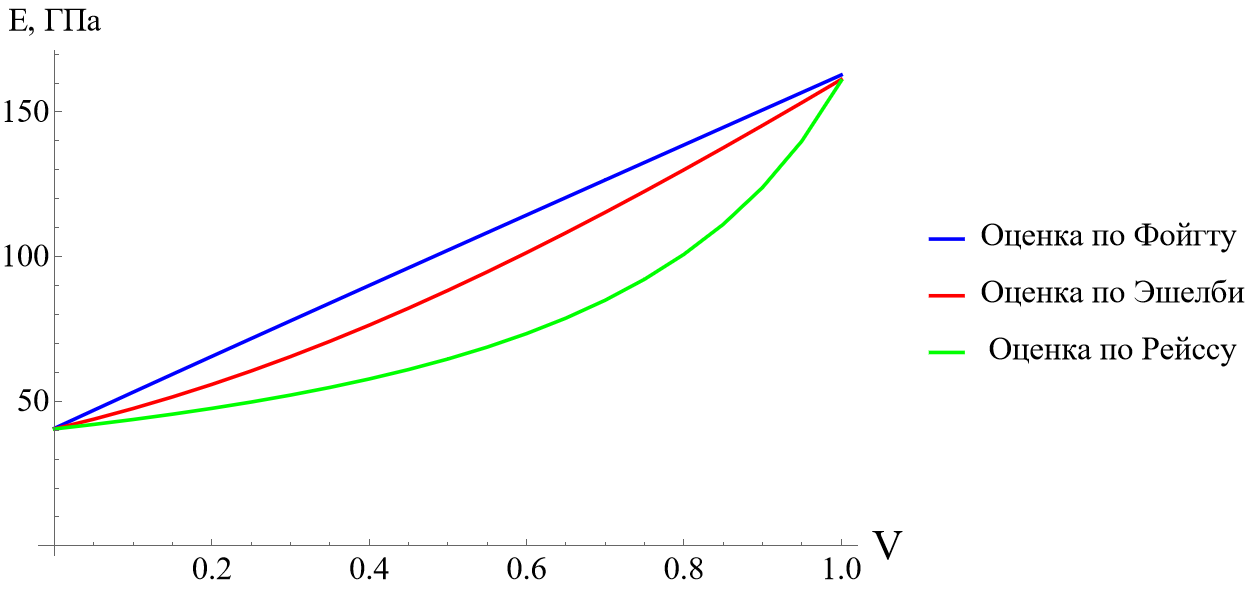
\includegraphics[width=0.7\textwidth]{e-p-1}%
	\caption{Оценки модуля Юнга пористого двухфазного сплава-смеси при $V_3 = 0$}
	\vspace*{-2mm}
	\label{puasson-pic-p-1}
\end{figure}
\begin{figure}[!htbp]
	\centering
	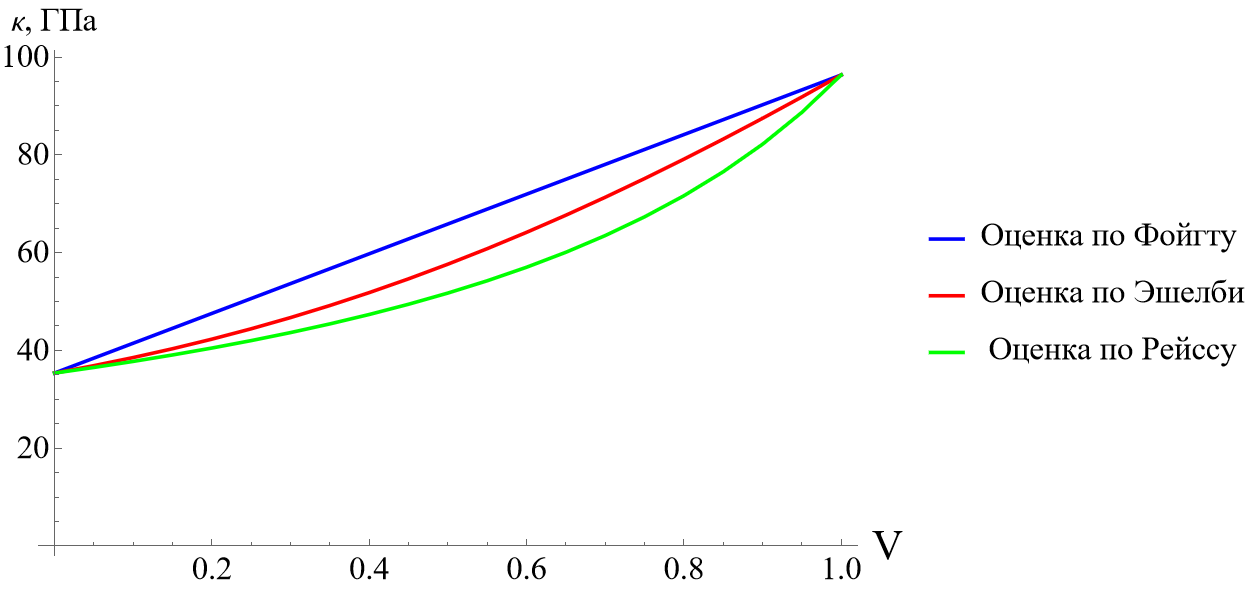
\includegraphics[width=0.7\textwidth]{k-p-1}%
	\caption{Оценки модуля объемной упругости пористого двухфазного сплава-смеси при $V_3 = 0$}
	\vspace*{-2mm}
	\label{puasson-pic-p-1}
\end{figure}
\begin{figure}[!htbp]
	\centering
	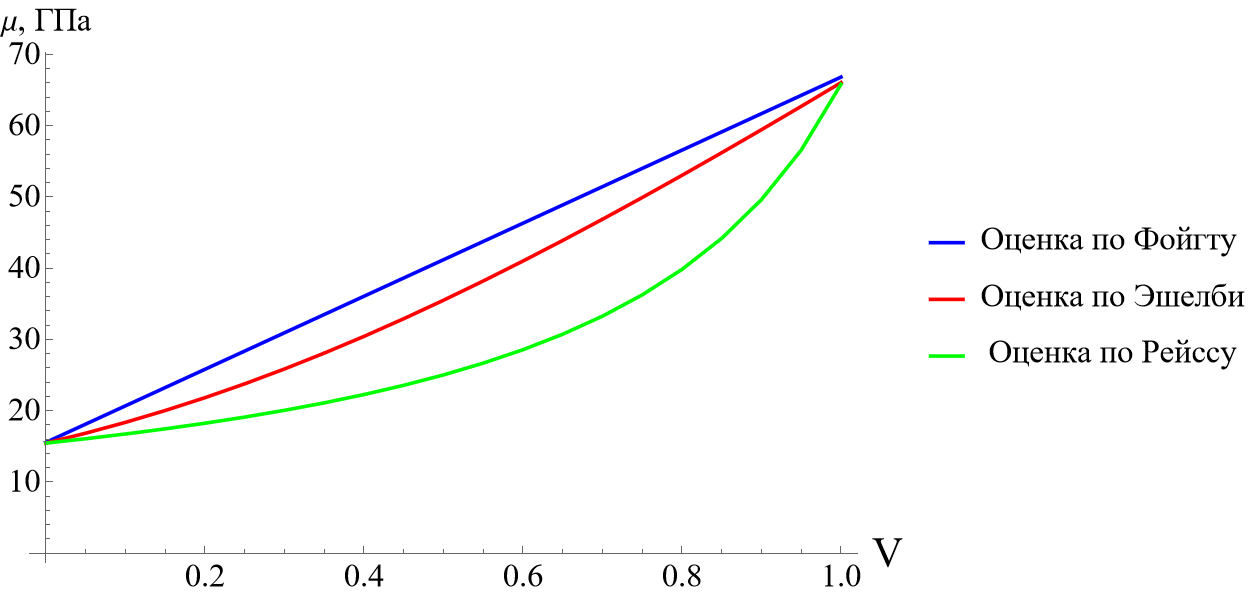
\includegraphics[width=0.7\textwidth]{nu-p-1}%
	\caption{Оценки модуля упругости пористого двухфазного сплава-смеси при $V_3 = 0$}
	\vspace*{-2mm}
	\label{puasson-pic-p-1}
\end{figure}
\begin{figure}[!htbp]
	\centering
	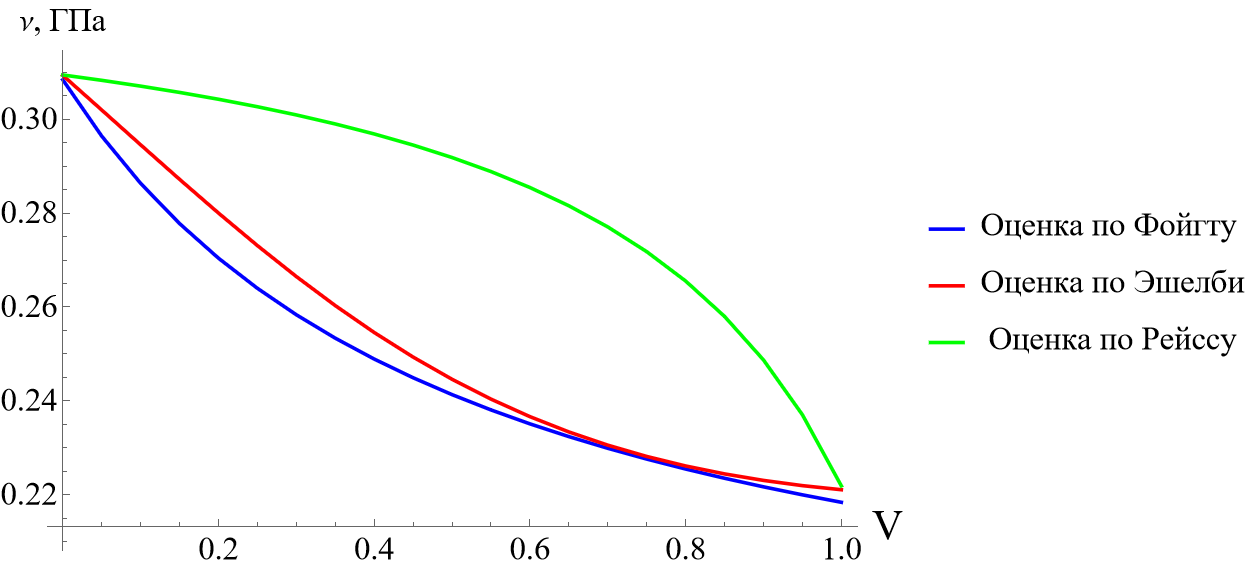
\includegraphics[width=0.7\textwidth]{v-p-1}%
	\caption{Оценки коэффициента Пуассона пористого двухфазного сплава-смеси при $V_3 = 0$}
	\vspace*{-2mm}
	\label{puasson-pic-p-1}
\end{figure}
\begin{figure}[!htbp]
	\centering
	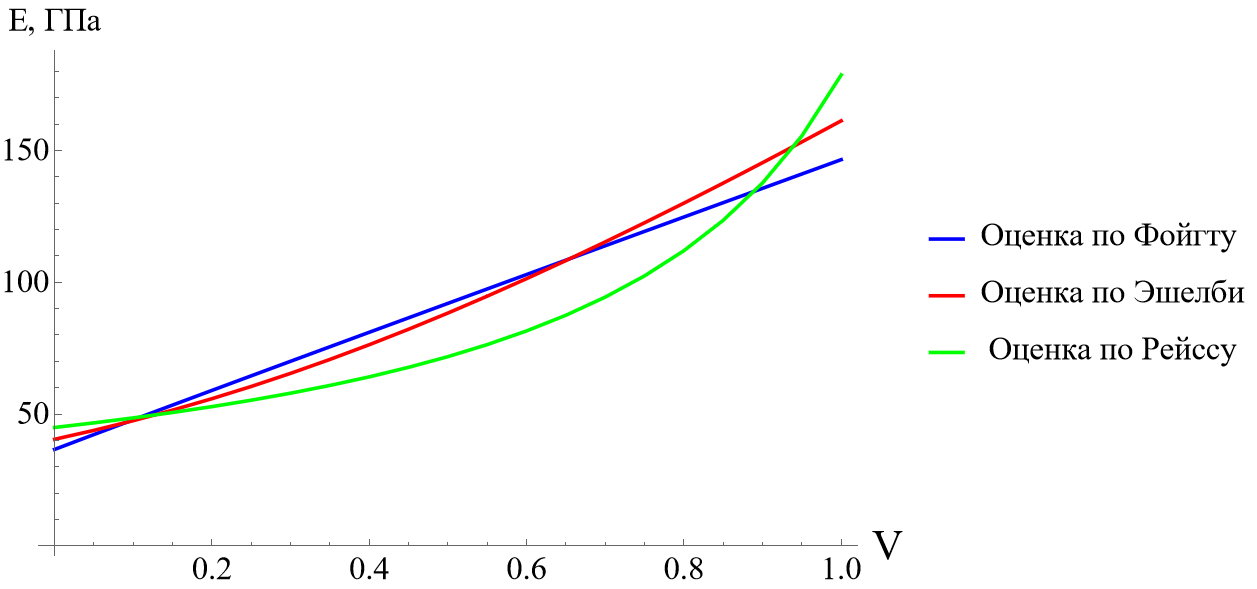
\includegraphics[width=0.7\textwidth]{e-p-2}%
	\caption{Оценки модуля Юнга пористого двухфазного сплава-смеси при $V_3 = 0.1$}
	\vspace*{-2mm}
	\label{puasson-pic-p-1}
\end{figure}
\begin{figure}[!htbp]
	\centering
	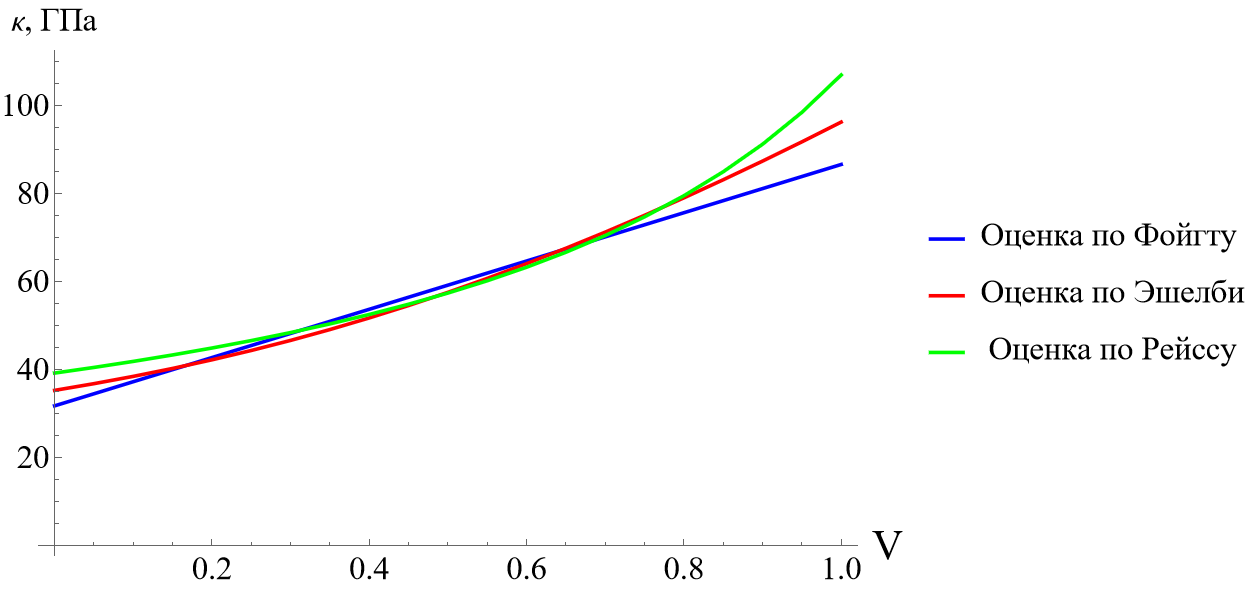
\includegraphics[width=0.7\textwidth]{k-p-2}%
	\caption{Оценки модуля объемной упругости пористого двухфазного сплава-смеси при $V_3 = 0.1$}
	\vspace*{-2mm}
	\label{puasson-pic-p-1}
\end{figure}
\begin{figure}[!htbp]
	\centering
	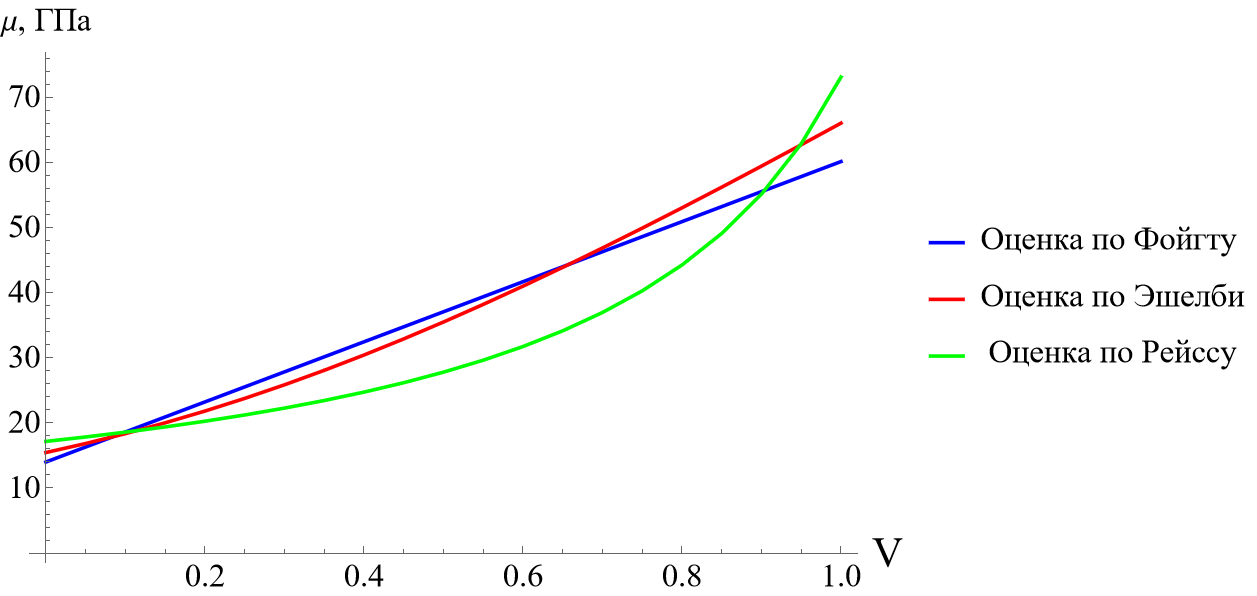
\includegraphics[width=0.7\textwidth]{nu-p-2}%
	\caption{Оценки модуля упругости пористого двухфазного сплава-смеси при $V_3 = 0.1$}
	\vspace*{-2mm}
	\label{puasson-pic-p-1}
\end{figure}
\begin{figure}[!htbp]
	\centering
	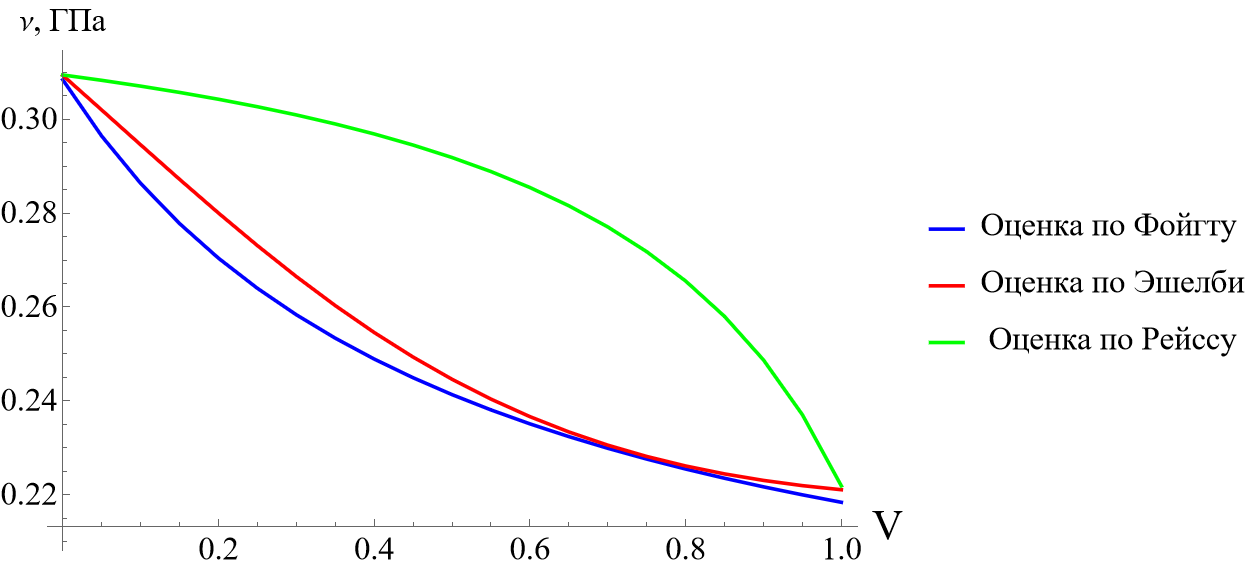
\includegraphics[width=0.7\textwidth]{v-p-2}%
	\caption{Оценки коэффициента Пуассона пористого двухфазного сплава-смеси при $V_3 = 0.1$}
	\vspace*{-2mm}
	\label{puasson-pic-p-1}
\end{figure}
\begin{figure}[!htbp]
	\centering
	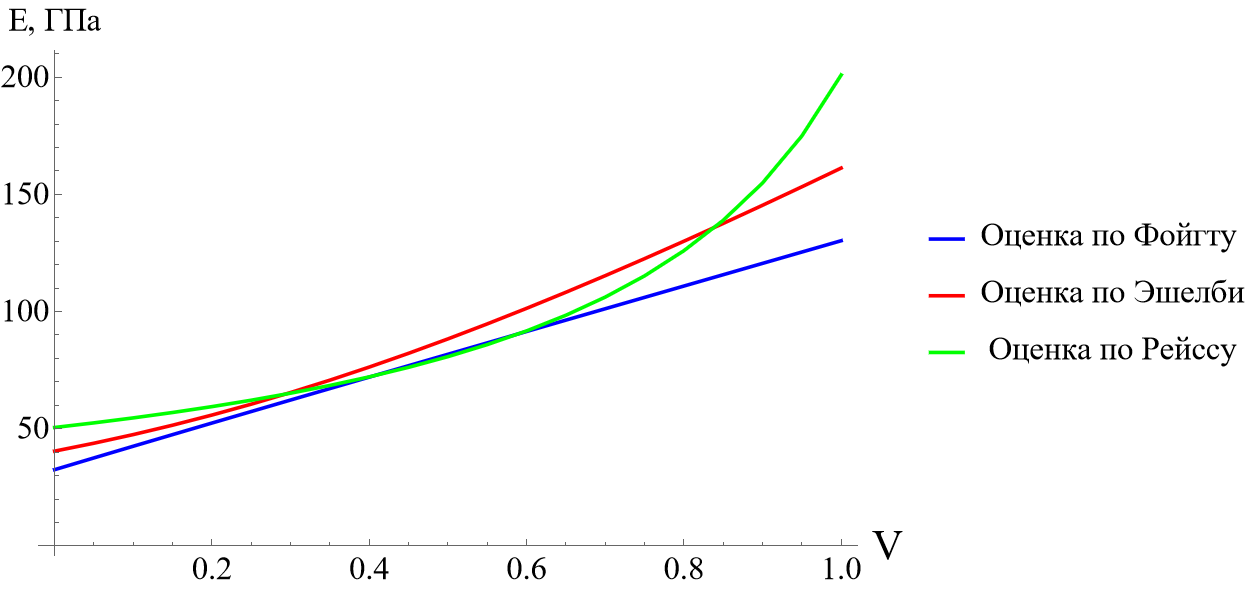
\includegraphics[width=0.7\textwidth]{e-p-3}%
	\caption{Оценки модуля Юнга пористого двухфазного сплава-смеси при $V_3 = 0.2$}
	\vspace*{-2mm}
	\label{puasson-pic-p-1}
\end{figure}
\begin{figure}[!htbp]
	\centering
	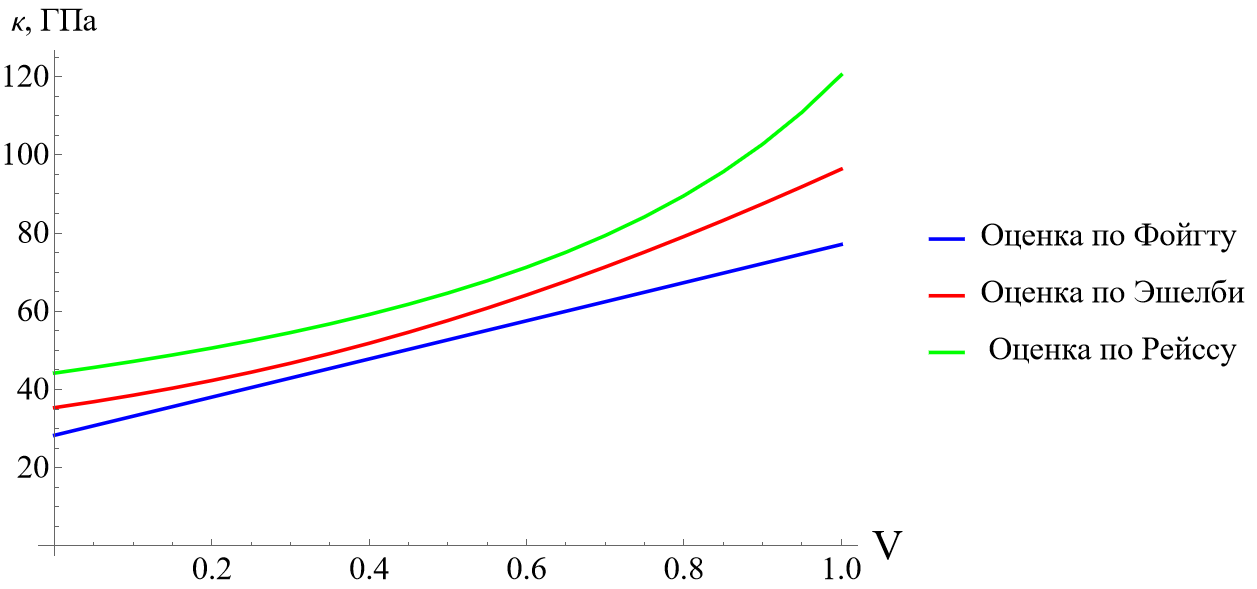
\includegraphics[width=0.7\textwidth]{k-p-3}%
	\caption{Оценки модуля объемной упругости пористого двухфазного сплава-смеси при $V_3 = 0.2$}
	\vspace*{-2mm}
	\label{puasson-pic-p-1}
\end{figure}
\begin{figure}[!htbp]
	\centering
	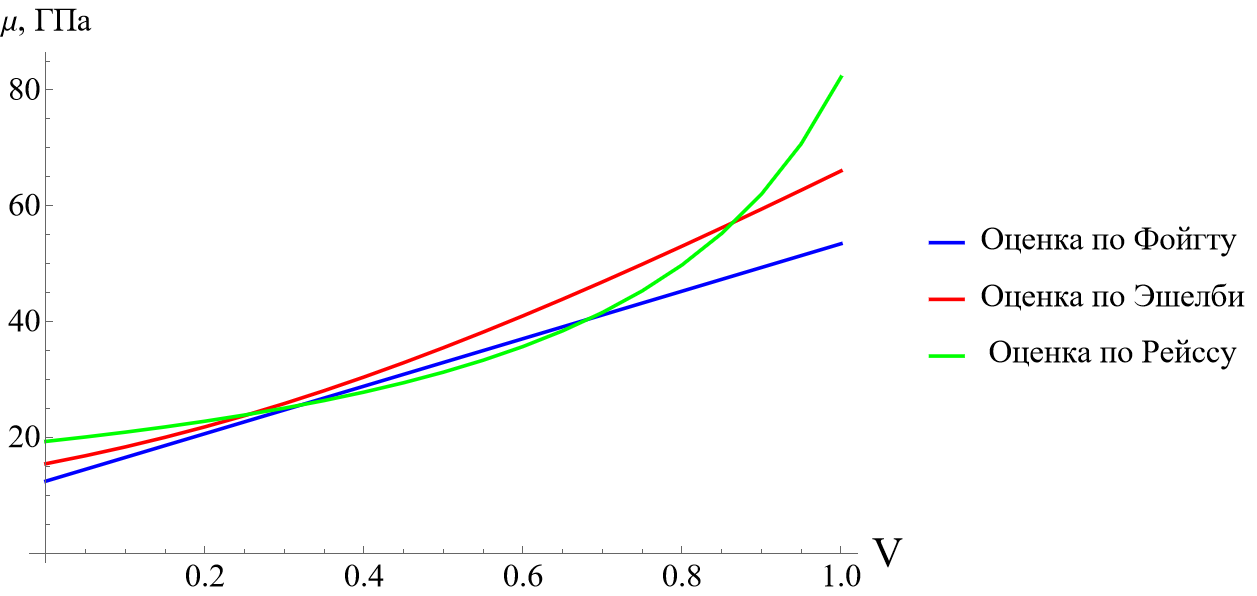
\includegraphics[width=0.7\textwidth]{nu-p-3}%
	\caption{Оценки модуля упругости пористого двухфазного сплава-смеси при $V_3 = 0.2$}
	\vspace*{-2mm}
	\label{puasson-pic-p-1}
\end{figure}
\begin{figure}[!htbp]
	\centering
	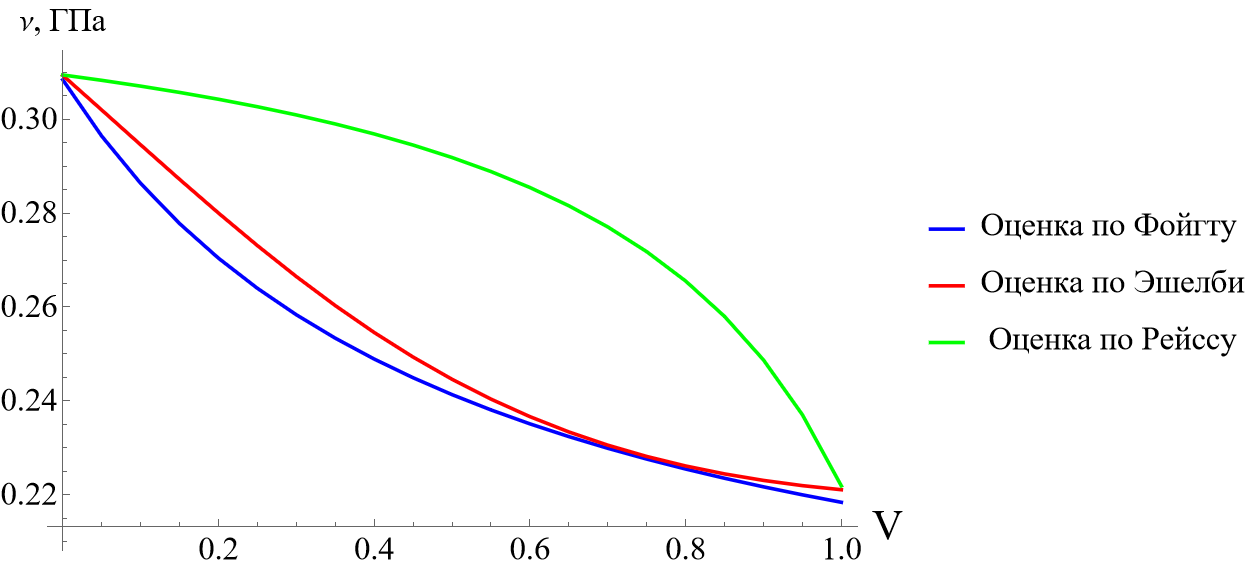
\includegraphics[width=0.7\textwidth]{v-p-3}%
	\caption{Оценки коэффициента Пуассона пористого двухфазного сплава-смеси при $V_3 = 0.2$}
	\vspace*{-2mm}
	\label{puasson-pic-p-1}
\end{figure}


\newpage
\section{Заключение}

В данной работе для заданной пары металлов были получены следующие результаты:
\begin{enumerate}
\item вычислены элементы матриц коэффициентов податливости и упругости;
\item построены графики зависимостей линейной податливости от направлений единичного вектора;
\item определенны направления, по которым линейная податливость имеет экстремальные значения;
\item найдены отношения полуосей эллипсоида вращения, образующегося после действия всестороннего давления на шар из металла с ГПУ-решеткой;
\item для поликристаллов найдены оценки по Фойгту и Рейссу коэффициента Пуассона в предположении хаотической ориентации зерен;
\item для поликристаллов найдены оценки для случая статистически усредненной шаровой формы кристаллических зерен (задача Эшелби)
\item проведены аналогичные расчеты для пористого двухфазного сплава-смеси из заданных металлов при трех фиксированных значения объемной пористости;
\item построены графики зависимостей коэффициента Пуассона от объемных долей металлов в сплаве.

\end{enumerate}

\newpage
\begin{thebibliography}{2}
\bibitem{first-zarubin} Зарубин В.С., Кувыркин Г.Н. Математические модели механики и электродинамики сплошной среды. М.: Изд-во МГТУ им. Н.Э. Баумана, 2008. 512 с.
\bibitem{second-zarubin} Зарубин В.С. Прикладные задачи термопрочности элементов конструкций. М.: Машиностроение, 1985. 296 с.
\bibitem{third-zarubin} Зарубин В.С. Физические и математические модели микромеханики: учеб-
ное пособие. В.С. Зарубин, Г.Н. Кувыркин, И.Ю. Савельева Москва: Издательство МГТУ им. Н.Э. Баумана, 2020. 194 с.

\end{thebibliography}

\end{document} 